\documentclass[12pt]{article}
\usepackage{fullpage}
\usepackage{subcaption,amsmath,amssymb,mathtools,xparse,graphicx,float,datetime,color,array,graphics,enumerate,tikz,pgfplots,xcolor}
\usepgfplotslibrary{statistics}
\pagestyle{empty}
\newcommand{\D}{\displaystyle}
\setlength{\textheight}{9in} \setlength{\headheight}{.2in}
\setlength{\headsep}{0in} \setlength{\topmargin}{0in}
\begin{document}
\begin{center}
CSCI 6100 Machine Learning From Data\\
Fall 2018\\
\end{center}
\begin{center}
HOMEWORK 6\\
Daniel Southwick\\
661542908\\
southd@rpi.edu
\end{center}
\vspace{.1in}

\noindent {\bf Exercise 3.4} \\\\
a) The in sample error is defined as: \begin{center} $\displaystyle E_{in}(w) = \frac{1}{N}||Xw - y||^2$\end{center} To minimize the sample error, we set the gradient of the sample error to 0: \begin{center} $\displaystyle \nabla E_{in}(w) = \frac{2}{N}(X^TXw - X^Ty)=0$\\$\displaystyle w = (X^TX)^{-1}X^Ty$
\begin{align*}	 
\hat{ {y}} &=  {X} {w} =  {X}( {X}^T {X})^{-1} {X}^T {y}\\
&=  {X}( {X}^T {X})^{-1} {X}^T( {X} {w}^*+\epsilon) \\
&=  {X} {w}^* +  X(X^TX)^{-1}X^T\epsilon\\
&=  {X} {w}^* +  {H}\epsilon
\end{align*} \end{center} 		
\indent b) The in sample error $\hat{y} - y$ can be expressed by:\begin{align*} \hat{ {y}}- {y} &= ( {X} {w}^* +  {H} {\epsilon}) - ( {X} {w}^*+ {\epsilon})\\ 
				&= ( {H}- {I}_{N}) {\epsilon}
\end {align*} Where $I_{N}$ denotes an $N\times N$identity matrix.\\\\
c) \begin{align*} \displaystyle E_{in}(w) &= \frac{1}{N}||(H-I_{N})\epsilon||^2 \\ &= \frac{1}{N}\epsilon^T(H - I_{N})^T(H-I_{N})\epsilon\end{align*} 
We know that $(H) - I_{N}$ is symmetric and $(H - I_{N})^2 = I_{N} - H$ by 3.3(c), thus:
\begin{center} $\displaystyle E_{in}(w) = \frac{1}{N}\epsilon^T(I_{N} - H)\epsilon$\end{center} \indent\\\indent\\\\\\
d) \begin{align*} \displaystyle\mathbb{E}_\mathcal{D}[E_{in}( {w})] &= \mathbb{E}_\mathcal{D}\left[\frac{1}{N}\  {\epsilon}^T {\epsilon} -\frac{1}{N}\  {\epsilon}^T {H} {\epsilon}\right]\\
&= \frac{1}{N}\ \mathbb{E}_\mathcal{D}\left[ {\epsilon}^T {\epsilon}\right] -\frac{1}{N}\ \mathbb{E}_\mathcal{D}\left[ {\epsilon}^T {H} {\epsilon}\right] \\
&= \frac{1}{N}(\ \mathbb{E}_\mathcal{D}\left[ {\epsilon}^T {\epsilon}\right] -\ \mathbb{E}_\mathcal{D}\left[ {\epsilon}^T {H} {\epsilon}\right] )
\end{align*}
Since $\epsilon$ is a noise term with zero means and $\sigma^2$, so $\ \mathbb{E}_\mathcal{D}\left[ {\epsilon}^T {\epsilon}\right] = N\sigma^2$, $\ \mathbb{E}_\mathcal{D}\left[ {\epsilon}^TH {\epsilon}\right]$ is a diagonal matrix, and $\ \mathbb{E}_\mathcal{D}\left[ {\epsilon}^T H {\epsilon}\right] =  trace(H)*\sigma^2$ and \begin{align*}
trace(H) &= trace(X(X^TX)^-1X^T) = trace((X^TX)^-1X^TX) \\ &=trace(I_{d+1}) = d+1
\end{align*} Where $I_{d+1}$ is a $d+1 \times \d+1$ dimension identity matrix. So 
\begin{align*} 
 \displaystyle\mathbb{E}_\mathcal{D}[E_{in}( {w})] &= \frac{1}{N}(N*\sigma^2 - (d+1)\sigma^2) \\ &= \sigma^2(1 - \frac{d+1}{N}) \end{align*}
e) \begin{align*}
\mathbb{E}_{\mathcal{D},   {\epsilon}^\prime}[E_{test}(  {w}_{lin})] 
			&= \mathbb{E}_{\mathcal{D},   {\epsilon}^\prime}\left[\ \frac{1}{N}\||Xw - y^\prime||^2 \right] \\
			&= \frac{1}{N}\mathbb{E}_{\mathcal{D},   {\epsilon}^\prime}\left[\ ||X(X^TX)^{-1}X^T(Xw^*+\epsilon) -(Xw^*+\epsilon^\prime)||^2 \right]\\
			&=\frac{1}{N}\mathbb{E}_{\mathcal{D}, {\epsilon}^\prime}\left[\ ||Xw^* + H\epsilon - (Xw^*+\epsilon^\prime) ||^2 \right]\\
			&=\frac{1}{N}\mathbb{E}_{\mathcal{D}, {\epsilon}^\prime}\left[\ ||H\epsilon - \epsilon^\prime ||^2 \right]\\
			&=\frac{1}{N}\mathbb{E}_{\mathcal{D}, {\epsilon}^\prime}\left[\ ||\epsilon^TH^TH\epsilon - 2\epsilon^TH^T\epsilon^\prime + (\epsilon^\prime)^T\epsilon^\prime||^2 \right]\\
			& = \frac{1}{N}(\sigma^2(d+1) + N\sigma^2)\\
			& = \sigma^2(1+\frac{d+1}{N})
\end{align*}\\
\newpage
\noindent {\bf Problem 3.1} \\\\
\indent In this Problem, we took the first semi-circle's coordinate center to be $(0,2.5)$ and the second center to be $(10,-2.5)$ to satisfy $rad = 10$, $thk = 5$ and $sep = 5$. \\\\
a) We first run the PLA starting from w = 0 until it converges, the final hypothesis came out to be $y = -0.001172x + 0.02945$\\\\
b) Then, we use the linear regression to obtain by $\displaystyle w = (X^TX)^{-1}X^TY = \left[-0.0416;0.0083;-0.0790\right]$ and the hypothesis came out to be $-0.0416+0.0083x-0.0790y=0$
\begin{figure}[H]
  \centering
  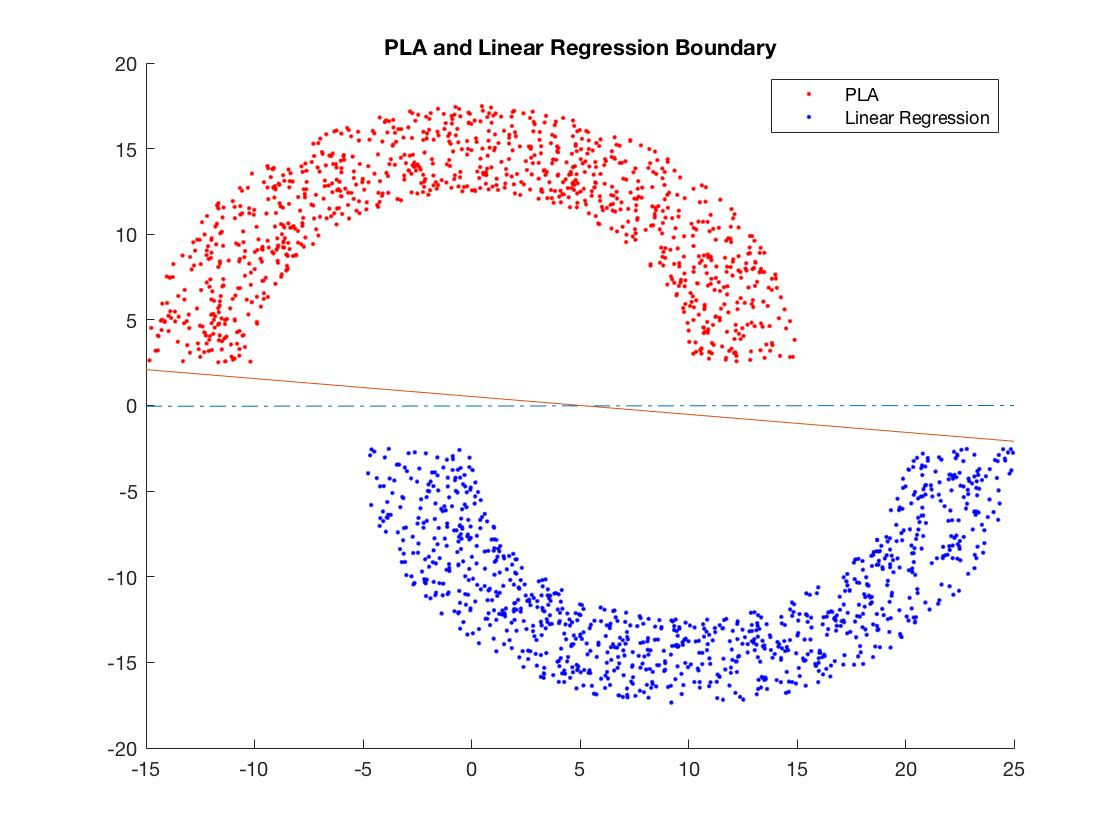
\includegraphics[scale = 0.35]{Pic1.jpg}
  \caption{PLA and Linear Regression final hypothesis result}
  \label{fig:Pic1}
\end{figure}
\indent Both PLA and linear regression hypothesis obtained in part a) and b) found solution to separate two regions. But the solutions generated from the different hypothesis are different. The result obtained by linear regression has the smallest $E_{in}$ comparing to PLA.\\

\newpage
\noindent {\bf Problem 3.2} \\\\
\indent We varied $sep$ in the range ${0.2,0.4,...,5}$ in the program from Problem 3.1 and run the PLA 25 times to record the number of iterations PLA takes to converge. Again, points are randomly sampled each time. 
\begin{figure}[H]
  \centering
  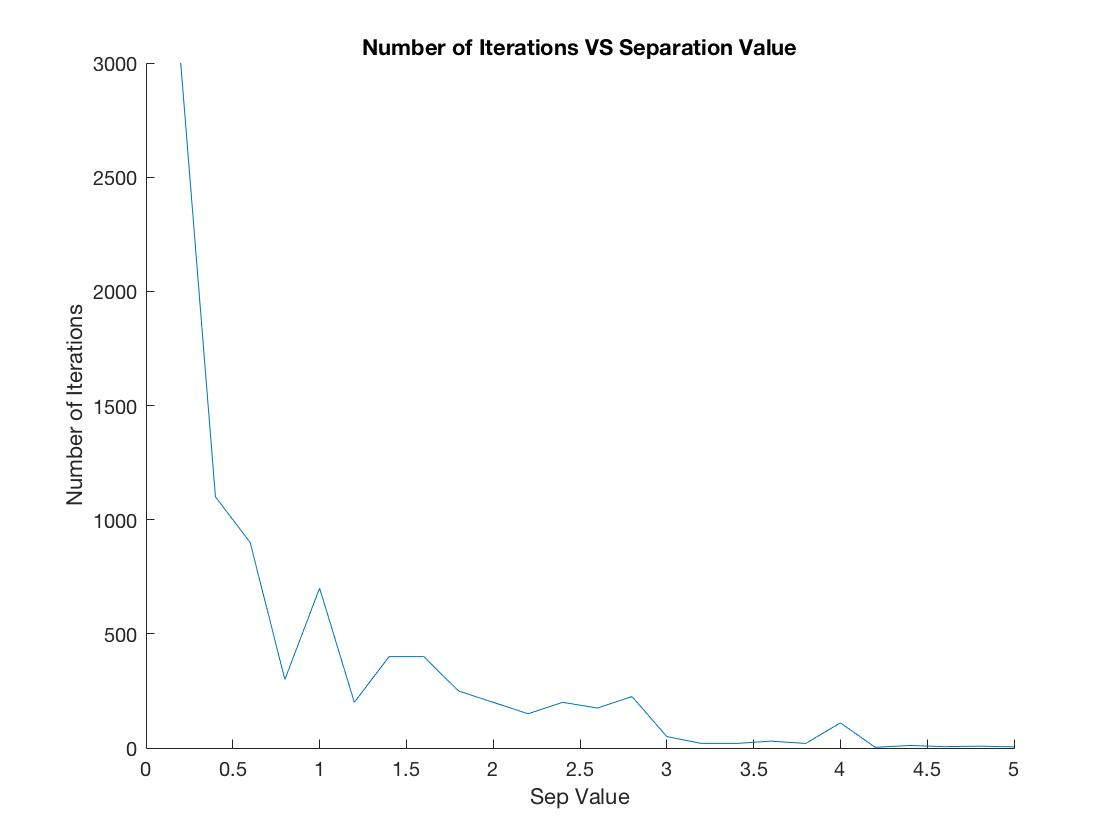
\includegraphics[scale = 0.35]{Pic2.jpg}
  \caption{Number of iterations PLA vs varies Sep Value}
  \label{fig:Pic2}
\end{figure}
\indent As $sep$ increases, the number of iterations decreases, we can interpret this intuitively, since two regions will be further away from each other, so PLA is much easier to converge. If one line can separate two regions for the smallest $sep$, it can also separate all regions with a larger parameter $sep$. So $R$ and $||w^*||$ are both constant, and $\rho$ increases with the increase of $sep$, the upper bound of iteration is $\displaystyle \frac{R^2||w^*||^2}{\rho^2}$, thus the number of iterations decrease as $sep$ increases.\\

\newpage
\noindent {\bf Problem 3.8} \\\\
\indent We know the out of sample error is: $E_{out}(h) = \mathbb{E}[(h( {x})-y)^2]$, to minimize $E_{out}(h)$, we can set it's gradient to 0,  by $\displaystyle \nabla E_{out}(h^*) = \mathbb{E}[h^*( {x})-y] = 0$ and for any fixed $x$, $h^*(x)$ can be treated as a fixed value, thus $\displaystyle h^*(x) = \mathbb{E}[y|x]$ by:
\begin{align*}\displaystyle
		\mathbb{E}[\mathbb{E}[X\big|Y]] 
		&= \sum_{y}\mathbb{E}[X\big|Y=y]\times P(Y = y) \\
		&= \sum_{y}\left(\sum_{x}x\times P\left(X = x\big|Y = y\right)\right)\times P(Y = y) \\
		&= \sum_{y}\sum_{x}x\times P\left(X = x\big|Y = y\right)\times P(Y = y) \\
		&= \sum_{y}\sum_{x}x\times P\left(Y = y\big|X = x\right)\times P(Y = y) \\
		&= \sum_{x}x\times P(X = x)\times\left(\sum_{y}P\left(Y = y\big|X = x\right)\right) \\
		&= \sum_{x}x\times P(X = x) \\
		&= \mathbb{E}[X]
\end{align*}
Thus : 
\begin{align*}
		\displaystyle \nabla E_{out}(h^*) &= \mathbb{E}[h^*( {x})-y] = 0 \\
		\mathbb{E}[y|x] & = \mathbb{E}[h^*(x)+\epsilon(x)|x]\\
		&=\mathbb{E}[h^*(x)|x]+\mathbb{E}[\epsilon(x)|x]\\
		\mbox{So } \mathbb{E}[\epsilon(x)|x] &= 0
\end{align*}
\indent Thus $\Rightarrow E_{out}$ is minimized at $h^*(x)$, the expected value $\epsilon(x)$ is zero.\\\\

\noindent {\bf Problem 3.6} \\\\
a)For linearly separable data, there must exist some $w$ that satisfy (separate the data correctly): \begin{center}
i) $y(i) = +1$, and $h(x(i)) = sign(w^Tx(i)) = +1$\\
ii)$y(i) = -1$, and $h(x(i)) = sign(w^Tx(i)) = -1$\end{center}
Either cases, $y(i)(w^Tx(i)) > 0$. Then we must be able to find an $\epsilon$ such that $y(i)(w^Tx(i)) \geq \epsilon$ for all data within the dataset. Now, we let $\displaystyle \hat{w} = \frac{w}{\epsilon}$, then:
\begin{center}
$\displaystyle y(i)(w^Tx(i)) = y(i)(\frac{w^Tx(i)}{\epsilon}) \geq \frac{\epsilon}{\epsilon} = 1$
\end{center}
Thus for some $w$, ie. $\displaystyle \hat{w} = \frac{w}{\epsilon}$, $y(i)(w^Tx(i)) \geq 1$ for all data.\\\\
b) Now we know that $y(i)(w^Tx(i)) \geq 1$, then $(y(i)x(i))^Tw \geq 1$ and $(-y(i)x(i))^Tw \leq -1$. We can construct the linear program as: 
\begin{center}
$\displaystyle A = -\left[y_1*x_1^T,y_2*x_2^T,...,y_n*x_n^T\right]_{n+1}^T$,$z = w$, $b = [-1,-1,...,-1]_{n+1}^T$\\\indent\\
For $\displaystyle \min_{z} c^Tz$ subject to $Az \leq b$
\end{center}
So if the given data set is linearly separable, then the LP problem is feasible, then the obtained $w$ can separate the dataset.\\\\
c) We can derive
\begin{align*}
y_n(w^Tx_n) & \geq 1 - \xi_n \\
(y_nx_n^T)w + \xi_n & \geq 1\\ 
(-y_nx_n^T)w - \xi_n & \leq -1
\end{align*}
Now, combining $-\xi_n \leq 0$, we can construct the linear program as:
\begin{center}
$A = \begin{bmatrix}
    -y_1*x_1^T  & -1 & 0 & \cdots & 0\\
    -y_2*x_2^T  & 0  & -1 & \cdots & 0 \\
    \vdots & \vdots & \vdots & \ddots & \vdots\\
    -y_n*x_n^T  & 0  & 0 & \cdots & -1 \\
    0 & -1 & 0 & \cdots & 0\\
    0 &  0 & -1 & \cdots & 0\\
    \vdots & \vdots & \vdots & \ddots & \vdots\\
    0 & 0  & 0 & \cdots & -1\\
\end{bmatrix}_{(n+1)\times 2n}$
$z = \begin{bmatrix}
w\\\xi_1\\ \xi_2\\ \vdots \\ \xi_n
\end{bmatrix}_{n+1}$
$b = \begin{bmatrix}
-1 \\ -1 \\ \vdots \\-1 \\0 \\0 \\ \vdots \\0
\end{bmatrix}_{2n}$
$c = \begin{bmatrix}
0 \\ 1 \\ 1 \\ \vdots \\1
\end{bmatrix}_{n+1}$
\end{center} \indent \\
d) Now we derive from the result from part b) again:\\
Note that $\xi_n$ should be the lower bound, $\xi_n = max(0,1-y_n(w^Tx_n))$\\
Then:
\begin{align*} \displaystyle
y_n(w^Tx_n) & \geq 1 - \xi_n \\
\xi_n & \geq 1 - y_n(w^Tx_n)\\ 
\mbox{So we can minimize:     }& \min_w \sum_{i = 1}^{N}\max (0,1-y_nw^Tx_n)
\end{align*}  Which is the same problem as 3.5

\newpage
\noindent {\bf Handwritten Digits Data -  Obtaining Features} \\\\
a)We've sorted out the number images and chose to display a number 1 and a number 5 here:
\begin{figure}[H]
\centering
\begin{subfigure}{.5\textwidth}
  \centering
   
\includegraphics[scale = 0.05]{1.jpg}
  \caption{Digit 1}
  \label{fig:1}
\end{subfigure}%
\begin{subfigure}{.5\textwidth}
  \centering
   
\includegraphics[scale = 0.05]{5.jpg}
  \caption{Digit 5}
  \label{fig:5}
\end{subfigure}
\caption{1 and 5}
\label{fig:test}
\end{figure}
b)Here we choose the features of intensity and symmetry, where symmetry in this case means the whether the image is vertical symmetry. Let $f(i,j)$ denotes the grayscale values from $-1$ to $1$ for pixel $(i,j)$ as given. And $i,j$ ranges from $1$ to $16$. Then the intensity is defined as:\begin{center} $\displaystyle I_{avg} = \frac{1}{256}\sum_{i = 1}^{16} \sum_{i = 1}^{16} f(i,j)$
\end{center}
Then the symmetric is defined as \begin{center} 
$\displaystyle I_{sym} = \frac{1}{256}\times\frac{1}{256}\sum_{i = 1}^{16} \sum_{i = 1}^{16} |f(i,j)-f(17-i,j)|$
\end{center}
c) We calculated $I_{avg}$ and $I_{sym}$ for all the $1$ and $5$ training data, the result is as follows, we can see that digit 5 has higher intensity and symmetrisity than digit 1.
\begin{figure}[H]
  \centering
  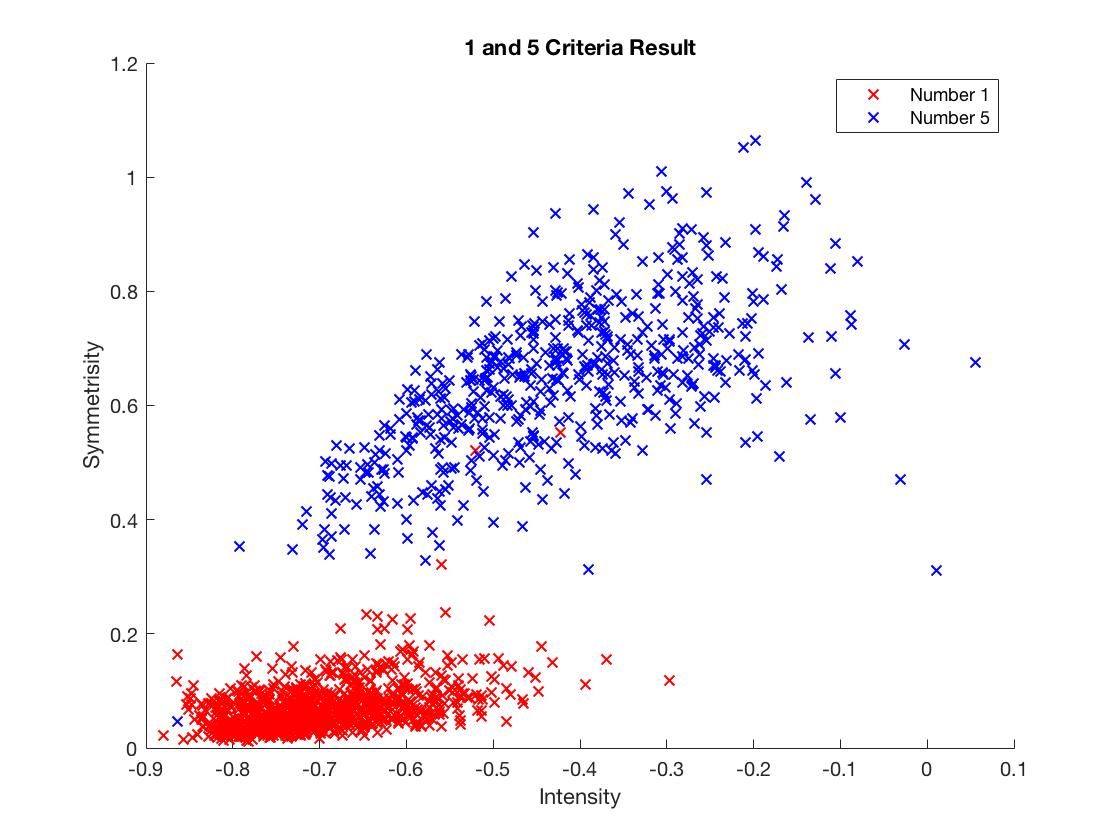
\includegraphics[scale = 0.3]{crit.jpg}
  \caption{Intensity and Symmetrisity Result for digit 1 and 5}
  \label{fig:Pic2}
\end{figure}
\end{document}
